% =====================================================================
%  Programming for AI & Data Science - Semester 261
%  Assignment report: day-ahead electricity load forecasting for Spain
%  Compiles with pdfLaTeX (needs the vntex package, available on Overleaf)
%  or with XeLaTeX / LuaLaTeX.
%  Red "TODO" boxes mark parts that are not done yet (search for \todo).
% =====================================================================
\documentclass[11pt,a4paper]{article}

\usepackage{iftex}
\ifPDFTeX
  \usepackage[utf8]{inputenc}
  \usepackage[T5]{fontenc}       % Vietnamese diacritics in member names
  \usepackage{lmodern}
\else
  \usepackage{fontspec}
\fi

\usepackage[margin=2.5cm]{geometry}
\usepackage{amsmath,amssymb,mathtools,bm}
\usepackage{booktabs,tabularx,array,multirow}
\usepackage{graphicx}
\graphicspath{{figures/}}
\usepackage{subcaption}
\usepackage{float}
\usepackage{xcolor}
\usepackage{enumitem}
\usepackage[numbers,sort&compress]{natbib}
\usepackage[hidelinks]{hyperref}
\usepackage[capitalise,noabbrev]{cleveref}

\setcounter{secnumdepth}{3}
\newcolumntype{Y}{>{\raggedright\arraybackslash}X}

% ---------- notation and helpers --------------------------------------
\newcommand{\todo}[1]{\textcolor{red}{\textbf{[TODO:} #1\textbf{]}}}
\newcommand{\code}[1]{\texttt{#1}}
\newcommand{\HDD}{\mathrm{HDD}}
\newcommand{\CDD}{\mathrm{CDD}}
\newcommand{\MAE}{\mathrm{MAE}}

\begin{document}
\begin{center}
\vspace{2em}
\begin{Large}
VietNam National University Ho Chi Minh City\\
Ho Chi Minh City University of Technology\\
Faculty of Computer Science and Engineering


\vspace{6em}

\includegraphics[width=0.25\linewidth]{figures/HCMUT.png} \\
\vspace{8em}
\textbf{
Programming for AI and Data Science (\todo{course code})\\
Assignment Report\\
\Huge Day-ahead Electricity Load Forecasting for Spain\\
}
\vspace{4em}
\textbf{\todo{class} Group \todo{group name}}
\begin{table}[h!]
  \centering
    \label{tab:table1}
    \begin{tabular}{ll}
    \textbf{Instructor} & \\
    \todo{instructor name}  & \\
    & \\

    \textbf{Student Name} & \textbf{Student ID} \\

    Phan Ba Thanh & 2353084 \\
    \todo{other members} & \\

    \end{tabular}
\end{table}

\end{Large}
\vspace*{\fill}

\end{center}
\clearpage

\tableofcontents
\clearpage

% =====================================================================
%  1. Problem Definition
% =====================================================================
\section{Problem Definition}
\label{sec:problem}

\subsection{Task}
\label{sec:task}

We forecast the hourly electricity load of Spain one day ahead. At 10:00 local time on day $D-1$,
two hours before the 12:00 gate closure of the day-ahead market, the model outputs 24 values
$\hat y_{D,0},\dots,\hat y_{D,23}$ in megawatts (MW), one for each local hour of day $D$. Only information
published before 10:00 on $D-1$ may be used. The newest load hour that is surely available at that
time is the hour stamped 08:00 on $D-1$. The most recent \emph{same-hour} load value is therefore
two days old ($D-2$), not one.

\subsection{Who needs it and what we ask}
\label{sec:questions}

The dataset already contains the forecast of the transmission system operator (TSO). If a user only
needs a number, the TSO column is the right choice, and our model does not try to replace it.
Our target user is an analyst who only has public data and wants an open, explainable model. Such a
user needs to know where to spend effort: on feature engineering, on a more complex model, or on
obtaining weather forecasts. We therefore ask three questions:
\begin{enumerate}[label=\textbf{Q\arabic*}, leftmargin=*]
  \item How much error do lag, calendar, holiday and temperature features remove, using a linear model
        (B1 Ridge versus the seasonal-naive B0)?
  \item Does a non-linear model (M1 LightGBM, Light Gradient Boosting Machine) add accuracy once these features exist (M1 versus B1)?
  \item How much is knowing the actual weather of day $D$ worth, compared with only past weather?
\end{enumerate}

\subsection{Dataset}
\label{sec:dataset}

We use the Kaggle dataset ``Hourly energy demand generation and weather''~\cite{jhana2019energy}.
It joins load and generation data from ENTSO-E (European Network of Transmission System Operators
for Electricity) with hourly weather of five Spanish cities
(\cref{tab:dataset}).

\begin{table}[H]
  \centering
  \small
  \caption{The two files of the dataset and what we use from them.}
  \label{tab:dataset}
  \begin{tabularx}{\linewidth}{@{}l l Y@{}}
    \toprule
    File & Size & Used columns \\
    \midrule
    \code{energy\_dataset.csv} & 35{,}064 hourly rows, 2015--2018, 29 columns
      & \code{total load actual} (target); \code{total load forecast} (TSO forecast, reference only).
        Generation and price columns are dropped because they are simultaneous with the target or
        published after the 10:00 cutoff. \\
    \code{weather\_features.csv} & 178{,}396 rows, 5 cities, 17 columns
      & \code{temp} of Madrid, Barcelona, Valencia, Seville and Bilbao. \\
    \bottomrule
  \end{tabularx}
\end{table}

\subsection{Two weather settings}
\label{sec:weather-settings}

The dataset has observed weather but no weather \emph{forecasts}. We therefore run every model in
two settings and never mix them inside one comparison:
\begin{itemize}
  \item \textbf{actual}: the observed temperature of day $D$ is used, as if a perfect weather
        forecast were available. This gives an optimistic bound.
  \item \textbf{lagged}: only weather observed up to 08:00 on $D-1$ is used. This is a genuine
        ex-ante forecast with lagged predictors~\cite{hyndman2021fpp3} and needs no weather feed.
        It gives a pessimistic bound.
\end{itemize}
Performance with a real weather forecast lies between the two bounds, but it cannot be measured with
this dataset.

% =====================================================================
%  2. Literature Review
% =====================================================================
\section{Literature Review}
\label{sec:literature}

% TODO (before submission): re-check every number below against the original tables
% (several were read through an extraction tool). Sources marked "abstract" in the comments were
% only read at abstract level: read at least Charlton & Singleton, Lloyd and Bouktif in full.

System-level load forecasting methods fall into five groups: classical time-series models,
regression with hand-crafted features, tree ensembles, pattern-based methods, and deep learning.
Results across papers often look contradictory. Most of these differences come from three
factors: the forecast horizon, whether past load is an input, and how weather is provided.

\subsection{Classical statistical baselines}
\label{sec:lit-classical}

Seasonal naive copies the load of the same hour one day or one week earlier. ARIMA (autoregressive integrated moving
average) and exponential smoothing (ETS) model the series itself. On 35 ENTSO-E countries in 2018, Smyl et al.\ report a day-ahead
mean absolute percentage error (MAPE) of 5.08\% for weekly naive, 3.30\% for ARIMA and 3.11\% for ETS~\cite{smyl2023esdrnn}. In
Portugal, weekly seasonal naive reaches 4.29\%~\cite{pelekis2023comparative}. Wang et al.\ conclude
that naive models are not useful as the main benchmark at the aggregate level~\cite{wang2016recency}.
We therefore keep seasonal naive only as a floor (B0).

\subsection{Regression with feature engineering}
\label{sec:lit-regression}

Linear and additive models with calendar, lagged load and temperature terms are the classic
approach. Fan and Hyndman use a semi-parametric additive model with calendar, lagged load and
temperature for the Australian market~\cite{fan2012semiparametric}. The winner of the Global Energy
Forecasting Competition 2012 (GEFCom2012) was a
refined multiple regression with separate models per zone, hour, season and day
type~\cite{charlton2014refined}. In Italy, a regularised linear model using only the previous day's
load is competitive with the TSO forecast once special days are excluded~\cite{incremona2021italian}.
For Spain, Pardo et al.\ find that heating and cooling degree days (HDD, CDD) and seasonality stay significant
after autoregressive terms, on daily data~\cite{pardo2002temperature}. These models are easy to
explain, but they depend on the analyst choosing the right functional form.

\subsection{Tree ensembles and gradient boosting}
\label{sec:lit-trees}

Tree ensembles learn thresholds and interactions themselves. In GEFCom2012, an ensemble that
included gradient boosting machines with little domain tuning ranked second~\cite{lloyd2014gefcom}.
Rubattu et al.\ use LightGBM with lagged and rolling temperature statistics as the most important
inputs; they note that gradient boosting cannot extrapolate a long-term trend, a problem in their
year-ahead round~\cite{rubattu2023electricity}. In Dang-Ha et al., a random forest with lagged load
ranked second on both datasets and was more stable across them than the best
method~\cite{dangha2017local}.

\paragraph{Regression versus boosting.}
The literature we read does not settle which is better. A feature-engineered regression won
GEFCom2012 while a boosting ensemble came second~\cite{hong2013gefcomwinners}, but a competition rank
is not a significance test, and the setting (US zones, backcasting and one-week forecasts) differs
from ours. We found no readable study comparing the two on hourly national load, day-ahead, with
weather. This is exactly the comparison of Q1 and Q2.

\subsection{Pattern-based methods and deep learning}
\label{sec:lit-dl}

Deep learning results are mixed. A meta-regression over 59 studies finds long short-term memory (LSTM) and hybrid networks
best overall~\cite{hopf2023meta}, and an LSTM beat tuned machine-learning models on French
load~\cite{bouktif2018optimal}. On the other hand, LSTM (2.76\% MAPE) was beaten by simple
pattern-based methods on 35 countries~\cite{smyl2023esdrnn}, and in Portugal a plain multilayer perceptron (MLP, 2.02\%)
was close to N-BEATS (Neural Basis Expansion Analysis for Time Series, 1.90\%) at much lower cost~\cite{pelekis2023comparative}. Pattern-based
methods~\cite{dudek2021ensembles} are cheap and strong, but they use no weather, so they cannot
answer Q3. We do not implement LSTM. This is a scope decision: the assignment allows classical
machine learning only, and our questions are about features and weather. It is not a claim that
deep learning is worse.

\subsection{Temperature, information sets and explanation}
\label{sec:lit-weather}

Load is U-shaped in temperature (heating when cold, cooling when hot). Recent temperature history
(lags and moving averages) improved forecasts by 18--21\% over a benchmark in
GEFCom2012~\cite{wang2016recency}. Temperature is strongly collinear with season and hour of
day~\cite{pelekis2023comparative}, so its own effect is hard to isolate.

Hyndman and Athanasopoulos define \emph{ex-ante} forecasts as those using only information
available in advance, and \emph{ex-post} forecasts as those using later information on the
predictors~\cite{hyndman2021fpp3}. Many academic studies use ex-post weather. This is why we report
the \emph{actual} and \emph{lagged} settings separately (\cref{sec:weather-settings}).

For explanation we use SHAP (SHapley Additive exPlanations)
values~\cite{lundberg2017unified}. TreeSHAP, the SHAP algorithm for tree ensembles, only partly accounts for
dependence between features, and explanations can be misleading when features are strongly
dependent~\cite{aas2021explaining}. SHAP explains what the \emph{model} uses, not how load depends
on its causes~\cite{chen2020true}. We therefore read SHAP by feature group, not by single feature.

\subsection{Summary and implications}
\label{sec:lit-summary}

\begin{table}[H]
  \centering
  \small
  \caption{Main lessons from the literature and how they shape our design.}
  \label{tab:lit-summary}
  \begin{tabularx}{\linewidth}{@{}Y Y@{}}
    \toprule
    Finding & Consequence for this work \\
    \midrule
    Seasonal naive is weak but standard~\cite{wang2016recency,smyl2023esdrnn}
      & B0 is a floor; the main opponent of LightGBM is a feature-engineered Ridge. \\
    Regression vs.\ boosting is unresolved~\cite{charlton2014refined,lloyd2014gefcom}
      & No expected winner is assumed; both outcomes are reported with confidence intervals. \\
    Degree days work for Spain~\cite{pardo2002temperature}; recency matters~\cite{wang2016recency}
      & Ridge gets HDD/CDD of current and 24-hour mean temperature. \\
    Boosting cannot extrapolate trends~\cite{rubattu2023electricity}
      & We check bias on validation and allow a ``change since last week'' target. \\
    Most studies use ex-post weather~\cite{hyndman2021fpp3}
      & Two weather settings, reported as optimistic and pessimistic bounds. \\
    Whether a TSO forecast can be beaten depends on the metric and on special-day
      handling~\cite{mobius2023better,incremona2021italian}
      & The TSO column is only a reference; we do not claim to beat or lose to it. \\
    SHAP is unreliable for dependent features~\cite{aas2021explaining,chen2020true}
      & Grouped SHAP, read as ``what the model uses''. \\
    \bottomrule
  \end{tabularx}
\end{table}


\section{Algorithm Implementation}
\label{sec:implementation}
% =====================================================================
%  3.1 Data cleaning and preprocessing
% =====================================================================
\subsection{Data Cleaning and Preprocessing}
\label{sec:preprocessing}

The test year 2018 is cut from the raw files before any processing, so not even a
forward-fill can carry test information into development. \Cref{tab:cleaning} lists each step and
the reason for it.

\begin{table}[H]
  \centering
  \small
  \caption{Cleaning steps. Counts refer to 2015--2017.}
  \label{tab:cleaning}
  \begin{tabularx}{\linewidth}{@{}p{2.6cm} Y Y@{}}
    \toprule
    Step & What we do & Why \\
    \midrule
    Time zone & Parse the \code{+01:00/+02:00} offsets as UTC (Coordinated Universal Time), convert to Europe/Madrid.
      & Demand follows the local clock; in UTC the morning peak would shift by one hour between
        winter and summer. \\
    Day $\times$ 24 grid & Spring-forward days get an empty 02:00 slot (not scored); the duplicated
      02:00 of autumn days is averaged.
      & Lags are looked up as ``same local hour, $k$ days ago''. A shift of 168 rows would be one
        hour off for a week after each clock change. \\
    Weather duplicates & Drop 3{,}076 duplicated (city, hour) rows; all duplicates carry identical
      temperatures (asserted in code).
      & Otherwise the merge multiplies rows. \\
    City names & Strip \code{" Barcelona"}. & A leading space creates a sixth ``city''. \\
    Units & Kelvin $\rightarrow$ $^\circ$C. & Readable degree-day bases. \\
    One-hour spikes & Set a load value to missing when it deviates by more than 15\% from the mean
      of its two neighbours while the neighbours agree within 10\%.
      & A national drop of 12\,GW (gigawatts) that recovers within one hour is a recording error. Thresholds of
        15, 20 and 25\% flag the same hours (3 in 2015--2017, 1 in 2018). \\
    Missing target & 34 raw missing hours plus the flagged spikes are never trained on or scored.
      & We do not score against invented values. \\
    Missing lag input & Forward-fill at most 3 hours.
      & Uses the past only; interpolation would use future values. \\
    Real outliers & Kept (midnight drops, holidays).
      & They are real events; the TSO forecast drops at the same hours. \\
    Weather aggregation & Simple mean of the five cities.
      & No external data needed and both models see the same variable. No population weights
        (limitation). \\
    \bottomrule
  \end{tabularx}
\end{table}

\paragraph{Time alignment.}
If timestamps mark the start of each hour, solar generation should peak around 13:00--14:00 local
time and temperature in mid-afternoon. \Cref{fig:alignment} confirms this: solar peaks at hour 13
and temperature at 16:00. Load and weather share the same time axis, so no shift is needed. Our
information cutoff (data up to hour 08 of $D-1$ for a 10:00 issue) is safe under either timestamp
convention.

\begin{figure}[H]
  \centering
  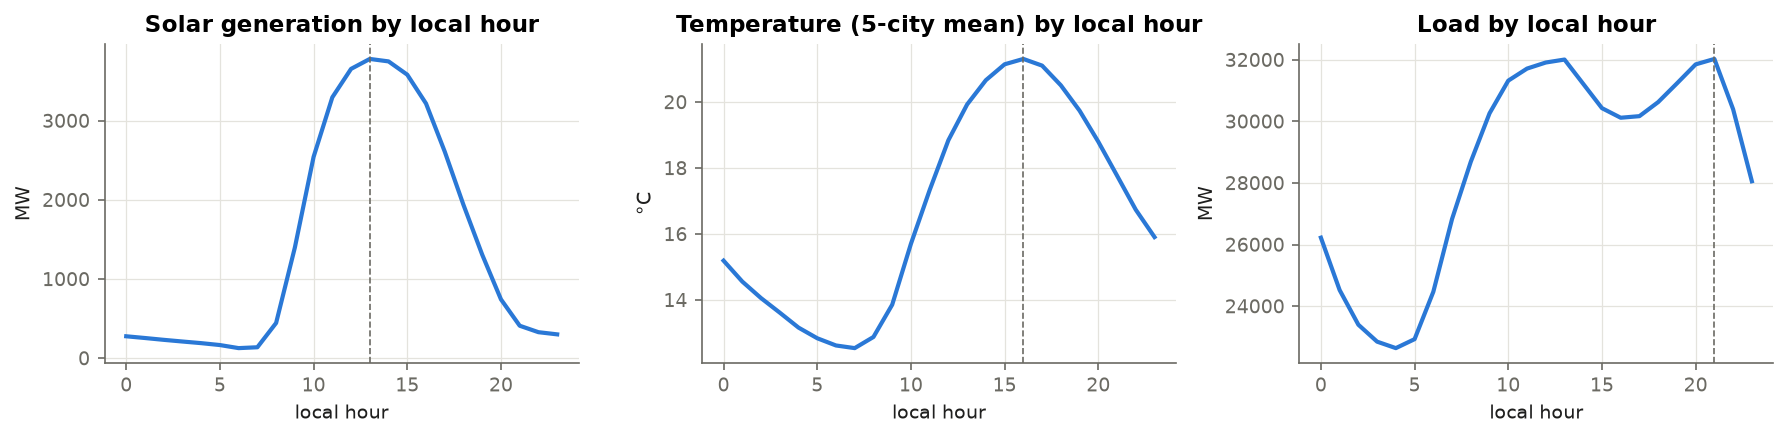
\includegraphics[width=\linewidth]{01_alignment_by_hour.png}
  \caption{Mean solar generation, temperature and load by local hour (2015--2017). Dashed lines mark
           the peak hour.}
  \label{fig:alignment}
\end{figure}

% =====================================================================
%  3.2 Exploratory data analysis (train years only)
% =====================================================================
\subsection{Exploratory Data Analysis}
\label{sec:eda}

The EDA uses only the training years 2015--2016, so that what we see cannot steer choices made on
validation.

\begin{figure}[H]
  \centering
  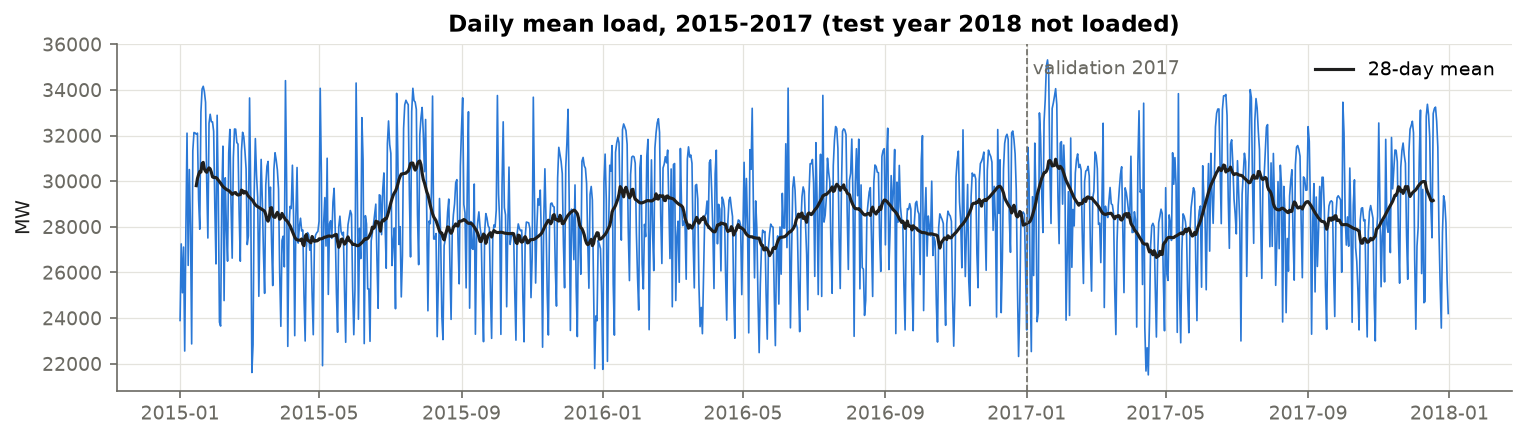
\includegraphics[width=\linewidth]{01_daily_load.png}
  \caption{Daily mean load with a 28-day moving average. The test year 2018 is not loaded.}
  \label{fig:daily-load}
\end{figure}

\Cref{fig:daily-load} shows a yearly cycle with winter and summer peaks, deep drops around
Christmas and in August, and a slow upward drift (annual means 28{,}391, 28{,}509 and 28{,}858\,MW
for 2015--2017).

\begin{figure}[H]
  \centering
  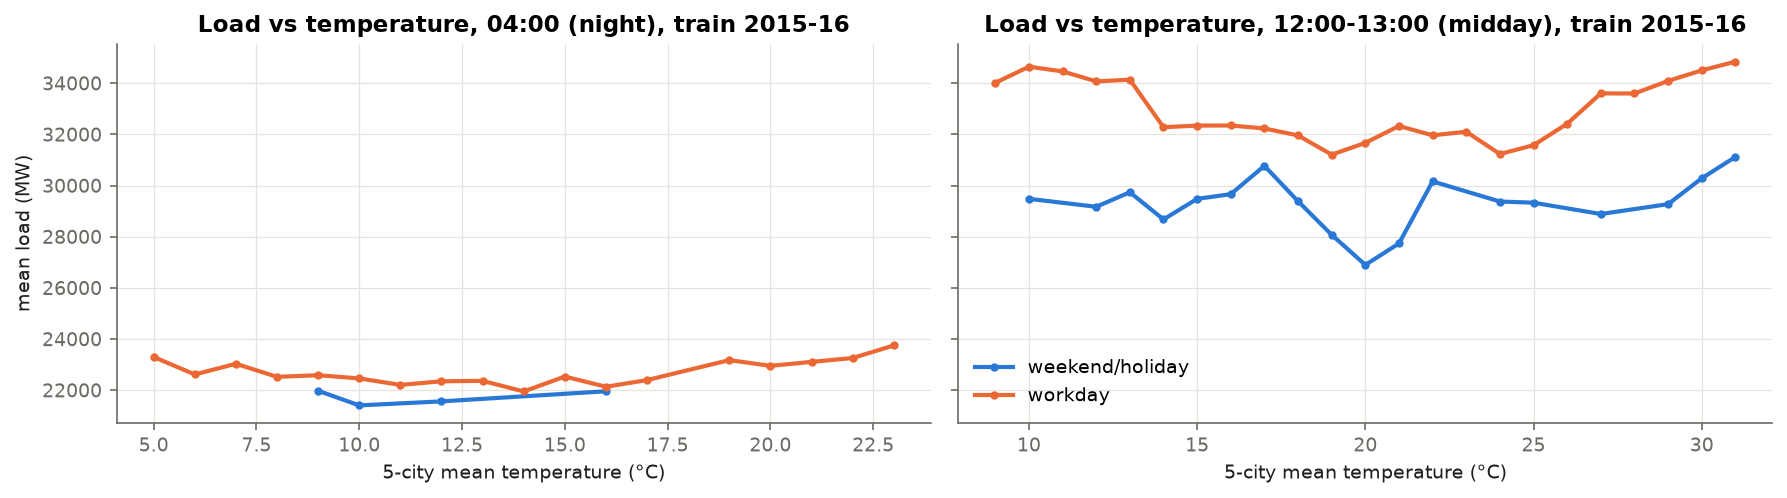
\includegraphics[width=\linewidth]{01_load_vs_temperature.png}
  \caption{Mean load per 1\,$^\circ$C temperature bin (bins with at least 15 hours), train years.}
  \label{fig:load-temp}
\end{figure}

At midday on workdays the U-shape is clear (\cref{fig:load-temp}): load is high below about
13\,$^\circ$C and above about 25\,$^\circ$C. At night the hot branch is weaker. However, cold
and hot days also differ in season, daylight and holidays, so this figure alone does not show that
temperature has its own effect.

\paragraph{Temperature effect within the same month.}
To remove the seasonal part we follow a rule fixed before looking at the data. Inside each cell of
hour $\times$ weekday $\times$ month $\times$ year (holidays and the Christmas window excluded), we
subtract the cell mean from both load and temperature and compute
$\beta=\sum \tilde y\,\tilde T/\sum \tilde T^2$. A branch passes if $\beta$ has the expected sign
(winter negative, summer positive) in \emph{both} years and its effect $|\beta|\,\mathrm{sd}(\tilde T)$
is at least 0.5\% of mean load. A second variant uses week instead of month cells.

\begin{table}[H]
  \centering
  \small
  \caption{Within-month temperature coefficient $\beta$ (MW/$^\circ$C) and effect of one standard
           deviation (\% of mean load), train years. A check mark means the year passes.}
  \label{tab:s2}
  \begin{tabular}{@{}l l rr rr@{}}
    \toprule
    & & \multicolumn{2}{c}{Month cells} & \multicolumn{2}{c}{Week cells} \\
    \cmidrule(lr){3-4}\cmidrule(l){5-6}
    Season & Year & $\beta$ & Effect & $\beta$ & Effect \\
    \midrule
    Winter (Dec--Feb) & 2015 & $+160$ & 1.24\% & $+76$ & 0.35\% \\
                      & 2016 & $-246$ & 1.88\% \checkmark & $-417$ & 1.59\% \checkmark \\
    July              & 2015 & $+79$ & 0.32\% & $+150$ & 0.55\% \checkmark \\
                      & 2016 & $+89$ & 0.59\% \checkmark & $-183$ & 0.96\% \\
    August            & 2015 & $-8$ & 0.04\% & $+154$ & 0.70\% \checkmark \\
                      & 2016 & $+440$ & 2.23\% \checkmark & $+572$ & 1.98\% \checkmark \\
    \bottomrule
  \end{tabular}
\end{table}

No branch passes in both years (\cref{tab:s2}). Winter 2015 has the wrong sign under both controls.
A possible reason is that most Spanish heating uses gas, so electric load reacts weakly to cold;
another is the quality of a five-city mean. Our data cannot separate the two. The summer effect is
mostly positive but small and unstable. We conclude that the U-shape in \cref{fig:load-temp} mostly
travels with the season. Temperature is still given to the models, but we do not claim a causal
``temperature drives load'' mechanism beyond seasonality.

% =====================================================================
%  3.3 Feature engineering
% =====================================================================
\subsection{Feature Engineering}
\label{sec:features}

Every feature of target hour $(D,h)$ uses only information available at 10:00 on $D-1$. The only
exception is the temperature of day $D$ in the \emph{actual} setting, which is allowed on purpose
(\cref{sec:weather-settings}). \Cref{tab:features} lists the features (\code{src/features.py}).

\begin{table}[H]
  \centering
  \small
  \caption{Features. Load lags are looked up by local date and hour, never by a shift in rows.}
  \label{tab:features}
  \begin{tabularx}{\linewidth}{@{}l p{4.6cm} Y@{}}
    \toprule
    Group & Feature & Why \\
    \midrule
    Load lags & $y_{D-2,h}$, $y_{D-7,h}$
      & Daily and weekly cycle; $D-2$ is the newest known value of the same hour. \\
      & $y_{D-1,08}$
      & Newest known hour: tells the current level after a sudden change (cold spell, start of a
        holiday). \\
      & mean($y_{D-1,0..8}$) / mean($y_{D-2,0..8}$) & Is the level rising or falling? \\
    Calendar & hour, weekday, month, $\sin$/$\cos$ of day of year & Daily, weekly, yearly cycles. \\
    Holidays & national flag; share of the 17 regions on holiday; bridge day; Dec 24--Jan 6 window
      & Holidays are where seasonal lags fail most. The regional share also captures days such as
        Holy Thursday (0.94). \\
      & regional share on $D-1$, $D-2$, $D-7$ & A lag taken from a holiday is a bad reference. \\
    Weather (actual) & $T_t$, mean of the last 24\,h & Current temperature and thermal inertia of
      buildings. \\
    Weather (lagged) & $T_{D-1,08}$, 24\,h mean ending at $D-1$ 08:00, $T_{D-2,h}$
      & Newest weather known at issue time. \\
    \bottomrule
  \end{tabularx}
\end{table}

Holidays come from the \code{holidays} package~\cite{holidays_python}, stored once as a CSV so that the
features do not depend on the package version. Ridge additionally receives degree days instead of
raw temperature (\cref{sec:models}); LightGBM receives raw temperature.

\paragraph{Automatic leakage test.}
For random days $D$, we replace \emph{all} load and temperature values after 08:00 on $D-1$ with
random noise, rebuild the features and assert that the features of day $D$ do not change. In the
\emph{actual} setting, only the temperature features of day $D$ are exempt. Over 8 random days per
setting the maximum change is exactly 0.

% =====================================================================
%  3.4 Data splitting
% =====================================================================
\subsection{Data Splitting}
\label{sec:splitting}

\begin{table}[H]
  \centering
  \small
  \caption{Chronological split. Random splits would leak future information into training.}
  \label{tab:split}
  \begin{tabularx}{\linewidth}{@{}l l r Y@{}}
    \toprule
    Set & Period & Usable hours & Why \\
    \midrule
    Train & 2015-01-08 -- 2016-12-31 & 17{,}332 & Two winters and two summers; the first week has no
      $y_{D-7,h}$. \\
    Validation & 2017 & 8{,}757 & A full year, so every season counts when choosing
      hyper-parameters. \\
    Test & 2018 & 8{,}756 & Touched once, after the configuration is frozen. \\
    \bottomrule
  \end{tabularx}
\end{table}

All hyper-parameters are chosen on validation with models fitted on 2015--2016. For the test, each
model is refitted \emph{once} on 2015--2017 with the frozen hyper-parameters and predicts all of
2018. This repeats the validation protocol (fit on earlier years, forecast the next full year), so
validation and test errors are comparable. Both weather settings use exactly the same rows, so all
models are scored on the same hours.

Two safeguards protect the test year. First, the development scripts never load 2018. Second, the
test script asserts that adding 2018 changes no feature of any earlier row, and it refuses to run
if the frozen parameters come from a smoke run or if the test has already been run.

% =====================================================================
%  3.5 Models
% =====================================================================
\subsection{Models}
\label{sec:models}

All models receive the same cleaned data and the same information for a given weather setting
(\code{src/models.py}).

\paragraph{B0: seasonal naive.} $\hat y_{D,h}=y_{D-7,h}$. It captures the daily and weekly cycle
for free. It is the floor every model must beat, not the main opponent.

\paragraph{B1: per-hour Ridge with degree days.}
Ridge regression~\cite{hoerl1970ridge} with standardised inputs (scaler fitted on training rows
only). Temperature enters through heating and cooling degree days
\begin{equation}
  \HDD(T)=\max(T_h-T,\,0), \qquad \CDD(T)=\max(T-T_c,\,0),
  \label{eq:degree-days}
\end{equation}
computed for each temperature feature, with separate bases $T_h\le T_c$ so that a flat comfort zone
is allowed. Weekday and month are one-hot encoded. We fit 24 separate models, one per local hour,
with a shared $\alpha$ and shared bases. With one shared $\alpha$, this is equivalent to a single Ridge
in which every feature interacts with the hour. It is the simplest way to let the effect of
temperature, weekday and lags differ between, for example, the 08:00 heating peak and the 15:00
cooling peak. We do \emph{not} interpret Ridge coefficients as ``MW per $^\circ$C'': they are shrunk
and shared between correlated features. Explanation uses SHAP on LightGBM instead.

\paragraph{M1: LightGBM.}
Gradient-boosted trees~\cite{ke2017lightgbm} with one \emph{global} model for all 24 hours, hour
being a feature. Each hour has only about 730 training days, and trees need many samples per leaf.
A global model can still split on the hour when the data support it. LightGBM receives raw
temperatures, since trees are invariant to monotone transforms and find thresholds themselves. Both
B1 and M1 minimise squared error, so the comparison is about the function class, not the loss.

\paragraph{Target option.}
The first validation run showed a bias of $-1.3\%$ of mean load in 2017. Our plan, written
before seeing any result, stated that a bias of at least 1\% triggers a second target option. Both
B1 and M1 can therefore predict either the level $y_{D,h}$ or the change since last week
$y_{D,h}-y_{D-7,h}$, and the choice is made on validation like any other hyper-parameter.

\paragraph{Additional variants (added after the first test run).}
Feedback from the lecturer pointed out that B0$\to$B1 changes two things at once, fitting a model
and engineering features, and that B1 (24 models) and M1 (one model) also differ in structure. We
therefore added five variants (\cref{tab:variants}) so that each question is answered by a pair that
differs in one thing only (\code{src/ablation.py}). \textbf{F0} is a minimal input set: hour, weekday,
month, the raw temperature of the setting ($T_t$ or $T_{D-1,08}$) and $y_{D-7,h}$, i.e.\ the
information B0 uses plus the calendar. It has no degree days, holidays, recent lags, morning ratio or
cyclic encodings. One-hot coding of weekday and month is kept for Ridge, because a linear model needs
it to use a category at all. \textbf{F1} is the full set of \cref{tab:features}. The global Ridge is
one model with hour dummies and no hour interactions; the per-hour LightGBM is 24 models sharing one
set of hyper-parameters, each with its own early stopping. All variants are tuned exactly like B1 and
M1 (\cref{sec:tuning}). For the global Ridge the best $\alpha$ fell on the upper edge of the grid
(one model on 24 times more rows needs a larger penalty), so the grid was extended by half decades,
as our rule prescribes; the chosen value lies inside the extended grid.

\begin{table}[H]
  \centering
  \small
  \caption{Model grid. Each variant exists in both weather settings.}
  \label{tab:variants}
  \begin{tabular}{@{}l l l l@{}}
    \toprule
    Model & Features & Structure & Status \\
    \midrule
    Ridge & F1 & 24 per-hour models & original B1 \\
    LightGBM & F1 & one global model & original M1 \\
    Ridge & F0 & 24 per-hour models & added \\
    Ridge & F0 & one global model & added \\
    Ridge & F1 & one global model & added \\
    LightGBM & F0 & one global model & added \\
    LightGBM & F1 & 24 per-hour models & added \\
    \bottomrule
  \end{tabular}
\end{table}

% =====================================================================
%  3.6 Hyper-parameter tuning
% =====================================================================
\subsection{Hyper-parameter Tuning}
\label{sec:tuning}

Every model is tuned on the same validation year, with validation MAE as the criterion, separately
in each weather setting. Budgets differ and are reported openly (\cref{tab:tuning}). Seed 42 is used
everywhere.

\begin{table}[H]
  \centering
  \small
  \caption{Tuning set-up.}
  \label{tab:tuning}
  \begin{tabularx}{\linewidth}{@{}l Y Y@{}}
    \toprule
    Model & Search space & Procedure \\
    \midrule
    B1 Ridge & target $\in$ \{level, change\}; $T_h\in\{10,\dots,20\}$, $T_c\in\{14,\dots,26\}$ (step
      2, $T_h\le T_c$); 11 values of $\alpha$ from $10^{-2}$ to $10^{3}$ (log scale)
      & Per target: bases at the middle $\alpha$, then $\alpha$ at the chosen bases. 94 fits per
        setting. The first $T_c$ grid started at 18 and its optimum lay on the edge, so the grid was
        widened before choosing. \\
    M1 LightGBM & target $\in$ \{level, change\}; \code{num\_leaves} 8--256; \code{min\_data\_in\_leaf}
      10--300; \code{feature\_fraction} 0.5--1; \code{lambda\_l2} $10^{-3}$--10
      & Optuna~\cite{akiba2019optuna} TPE, 30 trials. Learning rate fixed at 0.03; the number of trees
        comes from early stopping (200 rounds) on validation MAE and is kept fixed when refitting. A
        small budget on purpose: with two training years, heavy tuning overfits the validation
        year~\cite{smyl2023esdrnn}. \\
    \bottomrule
  \end{tabularx}
\end{table}

\paragraph{Ridge results.}
\Cref{tab:ridge-params} shows the chosen values. Both settings choose the change target and
$T_h=T_c=18\,^\circ$C, i.e.\ a V-shape with its minimum at 18\,$^\circ$C. The validation MAE is flat
around the optimum (all base pairs within about 30\,MW), so results do not hinge on the exact
bases. The $\alpha$ curves have an interior minimum (\cref{fig:ridge-alpha}).

\begin{table}[H]
  \centering
  \small
  \caption{Chosen Ridge hyper-parameters (validation 2017).}
  \label{tab:ridge-params}
  \begin{tabular}{@{}l l r r r r@{}}
    \toprule
    Setting & Target & $T_h$ & $T_c$ & $\alpha$ & Val.\ MAE (MW) \\
    \midrule
    actual & change & 18 & 18 & 31.6 & 1{,}839.5 \\
    lagged & change & 18 & 18 & 10.0 & 1{,}858.7 \\
    \bottomrule
  \end{tabular}
\end{table}

\begin{figure}[H]
  \centering
  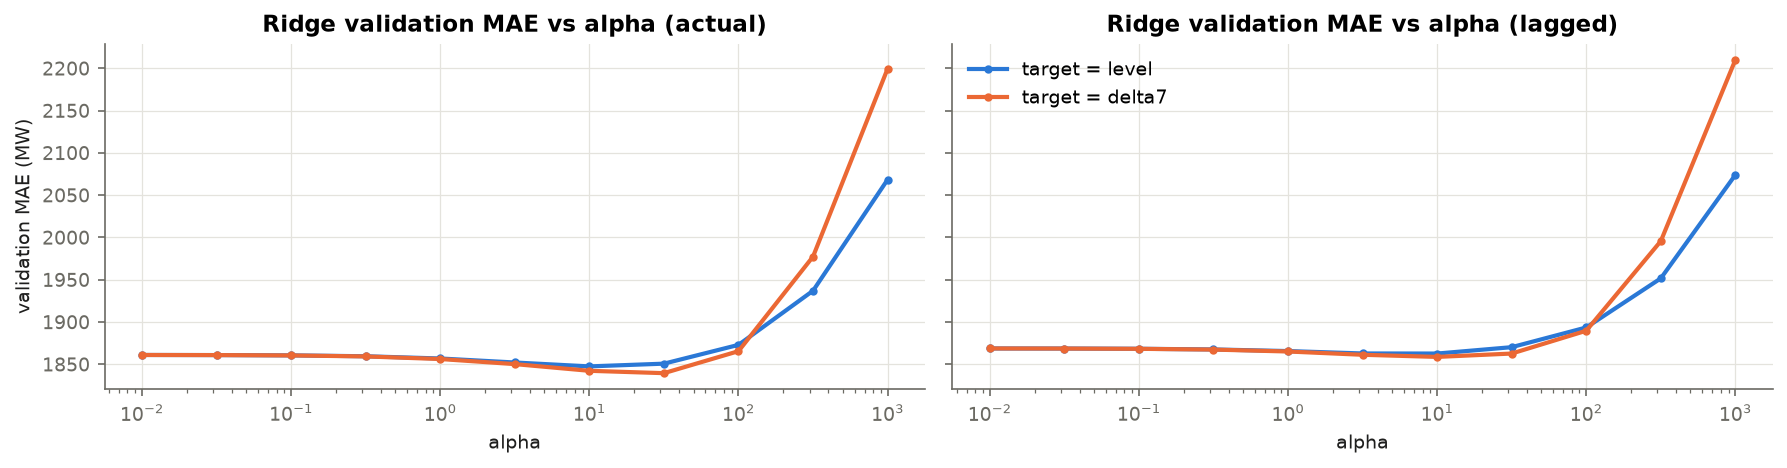
\includegraphics[width=\linewidth]{02_ridge_alpha.png}
  \caption{Ridge validation MAE against $\alpha$ for both target options.}
  \label{fig:ridge-alpha}
\end{figure}

\paragraph{LightGBM results.}
Tuning ran on a Kaggle CPU session (LightGBM 4.6.0, Optuna 5.0.0) in about 4 minutes per setting.
Both settings choose the level target: no trial with the change target came within 70\,MW of the
best level-target trial (\cref{fig:optuna}). The best-so-far curve is flat after trial 3 (actual) and trial 24 (lagged), so
30 trials are enough. The chosen models are large and lightly regularised (\cref{tab:lgbm-params}).
Because early stopping and model selection use the same validation year, the validation MAE of M1
is somewhat optimistic; the fair comparison is on the test year.

\begin{table}[H]
  \centering
  \small
  \caption{Chosen LightGBM hyper-parameters (validation 2017).}
  \label{tab:lgbm-params}
  \begin{tabular}{@{}l l r r r r r r@{}}
    \toprule
    Setting & Target & Leaves & Min.\ leaf & Feat.\ frac. & $\lambda_2$ & Trees & Val.\ MAE \\
    \midrule
    actual & level & 171 & 13 & 0.62 & 0.002 & 1{,}006 & 1{,}590.8 \\
    lagged & level & 70 & 11 & 0.55 & 0.46 & 2{,}153 & 1{,}683.4 \\
    \bottomrule
  \end{tabular}
\end{table}

\begin{figure}[H]
  \centering
  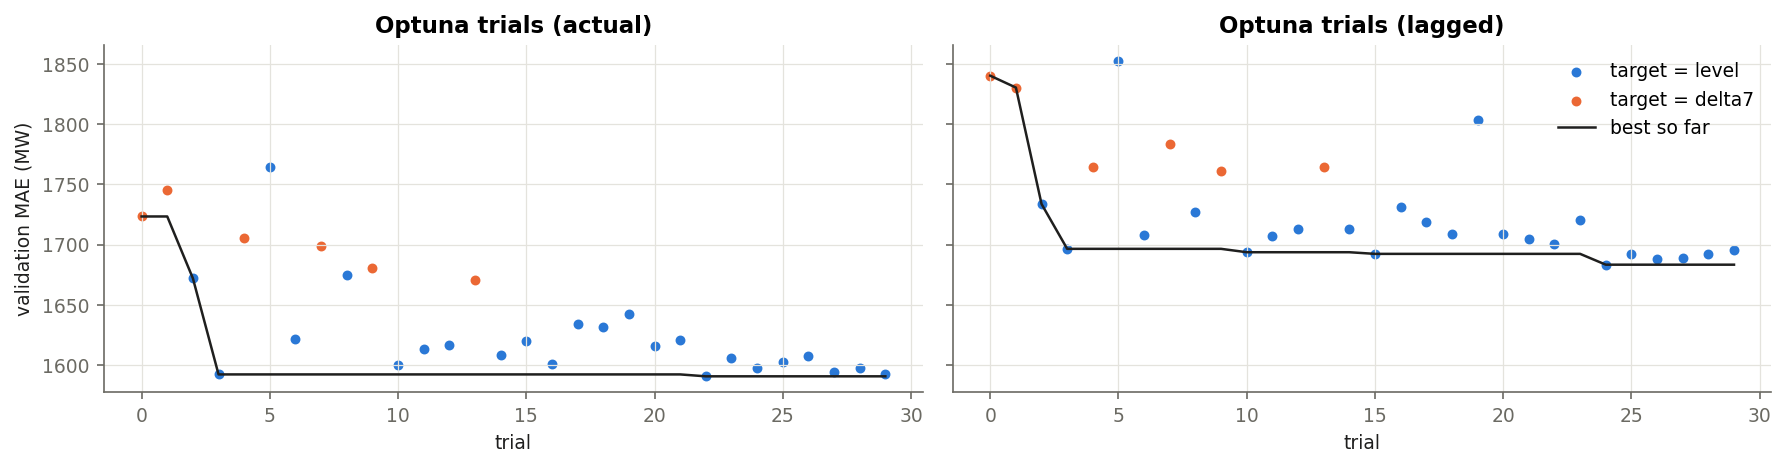
\includegraphics[width=\linewidth]{03_optuna_trials.png}
  \caption{Validation MAE of the 30 Optuna trials per setting, coloured by target option.}
  \label{fig:optuna}
\end{figure}

% =====================================================================
%  3.7 Model explanation
% =====================================================================
\subsection{Model Explanation}
\label{sec:explanation}

We explain M1 with TreeSHAP values from LightGBM's built-in \code{pred\_contrib}~\cite{lundberg2017unified}.
Lags, temperature, month and hour are correlated, and TreeSHAP handles such dependence only
partly~\cite{aas2021explaining}. We therefore sum SHAP values within four groups (load lags,
calendar, holidays, weather) and read them as ``what the model uses'', not as causal
effects~\cite{chen2020true}. We report:
\begin{itemize}
  \item mean $|\text{SHAP}|$ per group, overall and by month;
  \item the SHAP value of the weather group against temperature, at night and at midday, to see
        whether LightGBM learns the U-shape that Ridge receives through degree days.
\end{itemize}
If the change target is chosen, the SHAP values explain the predicted change since last week, not
the load level. Results are in \cref{sec:eval-shap}.


% =====================================================================
%  4. Evaluation
% =====================================================================
\section{Evaluation}
\label{sec:evaluation}

\subsection{Protocol}
\label{sec:protocol}

\paragraph{Metrics.} MAE in MW is the main metric because it has a physical unit. Root mean squared error (RMSE) stresses
large errors. MAPE is reported only for comparison with the literature, and is safe here because load
never approaches zero~\cite{hyndman2021fpp3}. We also report the bias (mean of prediction minus
actual).

\paragraph{Paired comparison.} For models A and B, let $\Delta=\MAE_A-\MAE_B$ (negative means A is
better). Errors of neighbouring hours are strongly autocorrelated, so we resample whole calendar
weeks (2{,}000 block-bootstrap samples~\cite{kunsch1989jackknife}) of the paired differences
$|e_A|-|e_B|$ and take the 95\% percentile interval. With a threshold $\delta$ equal to 2\% of the MAE
of the simpler model of the pair (a heuristic fixed before running the test), the verdict is:
\begin{itemize}
  \item \textbf{clearly better}: the interval excludes 0 and $|\Delta|\ge\delta$;
  \item \textbf{about equal}: the interval lies inside $[-\delta,+\delta]$;
  \item \textbf{undecided}: otherwise.
\end{itemize}
We also count in how many calendar months A beats B, to see whether a gain is broad or comes from a
few weeks.

\paragraph{TSO reference.} The TSO forecast is shown for context only. The TSO has internal data and
weather forecasts, and we do not know exactly when the column was last updated. We therefore do not
claim to beat or lose to it.

\subsection{Validation Results (2017)}
\label{sec:eval-val}

\begin{table}[H]
  \centering
  \small
  \caption{Validation 2017, 8{,}757 hours. Mean load 28{,}858\,MW.}
  \label{tab:val}
  \begin{tabular}{@{}l l r r r r@{}}
    \toprule
    Model & Weather & MAE & RMSE & MAPE (\%) & Bias \\
    \midrule
    B0 seasonal naive & -- & 2{,}627 & 3{,}748 & 9.20 & $-2$ \\
    B1 Ridge & actual & 1{,}840 & 2{,}562 & 6.38 & $-358$ \\
    B1 Ridge & lagged & 1{,}859 & 2{,}594 & 6.44 & $-378$ \\
    M1 LightGBM & actual & 1{,}591 & 2{,}350 & 5.56 & $-316$ \\
    M1 LightGBM & lagged & 1{,}683 & 2{,}438 & 5.89 & $-266$ \\
    \midrule
    TSO (reference) & -- & 314 & 430 & 1.08 & 2 \\
    \bottomrule
  \end{tabular}
\end{table}

\begin{table}[H]
  \centering
  \small
  \caption{Paired comparisons on validation ($\Delta$ in MW, 95\% block-bootstrap interval).}
  \label{tab:val-pairs}
  \begin{tabular}{@{}l l r c c l@{}}
    \toprule
    A & B & $\Delta$ & 95\% interval & Months A better & Verdict \\
    \midrule
    B1 actual & B0 & $-787$ & $[-1045,\,-512]$ & 12/12 & clearly better \\
    B1 lagged & B0 & $-768$ & $[-1036,\,-482]$ & 12/12 & clearly better \\
    B1 actual & B1 lagged & $-19$ & $[-54,\,17]$ & 8/12 & undecided \\
    M1 actual & B1 actual & $-249$ & $[-354,\,-134]$ & 12/12 & clearly better \\
    M1 lagged & B1 lagged & $-175$ & $[-275,\,-71]$ & 10/12 & clearly better \\
    M1 actual & M1 lagged & $-93$ & $[-153,\,-31]$ & 12/12 & clearly better \\
    \bottomrule
  \end{tabular}
\end{table}

On validation, features plus a linear model remove about 30\% of the seasonal-naive error, in every
month. LightGBM removes a further 9--14\% of the Ridge error. Knowing the actual weather helps
LightGBM by 93\,MW but Ridge by only 19\,MW, which is not distinguishable from zero. A possible
reading is that the trees use same-day temperature in a way the degree-day form does not, but this
is not shown yet (\cref{sec:eval-why}).

\paragraph{Resolution.} The half-width of the intervals is 100--110\,MW for M1 versus B1 and
35--60\,MW for actual versus lagged, against thresholds $\delta$ of about 34--37\,MW. Differences
smaller than roughly 100\,MW between models therefore end up ``undecided''. We keep $\delta$
unchanged and state this limit.

\paragraph{Loss versus metric.} Both models train on squared error but are scored by MAE. Removing
the median residual would lower the MAE by 30--50\,MW for both models (e.g.\ 1{,}840 to 1{,}791 for
B1 actual, 1{,}591 to 1{,}554 for M1 actual), so the mismatch affects both models by a similar
amount. This is only a diagnostic; predictions are not corrected.

\begin{table}[H]
  \centering
  \small
  \caption{Validation MAE (MW) by day type. Bold: best of B1/M1 in each weather setting.}
  \label{tab:val-daytype}
  \begin{tabular}{@{}l r r r r r r r@{}}
    \toprule
    Day type & Hours & B0 & B1 actual & M1 actual & B1 lagged & M1 lagged & TSO \\
    \midrule
    Workday & 5{,}950 & 2{,}583 & 1{,}778 & \textbf{1{,}453} & 1{,}802 & \textbf{1{,}553} & 307 \\
    Saturday & 1{,}248 & 2{,}230 & 1{,}606 & \textbf{1{,}541} & 1{,}662 & \textbf{1{,}615} & 316 \\
    Sunday & 1{,}271 & 2{,}974 & 2{,}194 & \textbf{1{,}955} & 2{,}152 & \textbf{2{,}089} & 308 \\
    Holiday & 240 & 4{,}193 & \textbf{2{,}957} & 3{,}451 & \textbf{2{,}984} & 3{,}278 & 466 \\
    Bridge day & 48 & 1{,}439 & \textbf{574} & 1{,}082 & \textbf{634} & 916 & 518 \\
    \bottomrule
  \end{tabular}
\end{table}

LightGBM wins on ordinary days but loses to Ridge on holidays and bridge days
(\cref{tab:val-daytype}). These days are rare (288 hours in the validation year and similarly few in
training), so the trees see few examples. Ridge treats the holiday share as one linear shift per hour,
which generalises from few examples. On the test year this holds only for bridge days
(\cref{sec:eval-why}).

The largest bias is in June 2017 ($-1{,}643$\,MW for B1 actual, $-956$\,MW for M1 actual), the month
of a record heat wave: June load was about 2{,}000\,MW above the June level of the two training
years. With only two training summers, the models had not seen such heat in June. We did not add
features to fix this after seeing the validation year, since that would overfit validation.

\subsection{Test Results (2018)}
\label{sec:eval-test}

The test script ran once on Kaggle (started 2026-11-10 17:16 UTC, after the configuration was frozen
at 16:32 UTC). It verified the SHA-256 (Secure Hash Algorithm) hashes of the frozen parameters and that adding 2018 changed
no feature of any earlier row. One one-hour spike in 2018 (6 May, 12:00) was set to missing by the
cleaning rule; 4 weather hours (clock-change slots) were forward-filled.

\begin{table}[H]
  \centering
  \small
  \caption{Test 2018, 8{,}756 hours (MW). The last column is the change from validation to test.}
  \label{tab:test}
  \begin{tabular}{@{}l l r r r r r@{}}
    \toprule
    Model & Weather & MAE & RMSE & MAPE (\%) & Bias & $\Delta$ vs.\ val. \\
    \midrule
    B0 seasonal naive & -- & 2{,}632 & 3{,}804 & 9.08 & $+13$ & $+5$ \\
    B1 Ridge & actual & 1{,}752 & 2{,}510 & 5.95 & $-402$ & $-88$ \\
    M1 LightGBM & actual & \textbf{1{,}521} & \textbf{2{,}286} & \textbf{5.18} & $-387$ & $-70$ \\
    B1 Ridge & lagged & 1{,}760 & 2{,}525 & 5.96 & $-445$ & $-99$ \\
    M1 LightGBM & lagged & 1{,}592 & 2{,}316 & 5.42 & $-355$ & $-92$ \\
    \midrule
    TSO (reference) & -- & 268 & 367 & 0.92 & $+2$ & $-46$ \\
    \bottomrule
  \end{tabular}
\end{table}

\begin{table}[H]
  \centering
  \small
  \caption{Paired comparisons on the test year ($\Delta$ in MW, 95\% block-bootstrap interval).}
  \label{tab:test-pairs}
  \begin{tabular}{@{}l l r c r c l@{}}
    \toprule
    A & B & $\Delta$ & 95\% interval & \% load & Months A better & Verdict \\
    \midrule
    B1 actual & B0 & $-880$ & $[-1120,\,-649]$ & $-3.0$ & 12/12 & clearly better \\
    B1 lagged & B0 & $-872$ & $[-1124,\,-632]$ & $-3.0$ & 12/12 & clearly better \\
    M1 actual & B1 actual & $-231$ & $[-342,\,-119]$ & $-0.8$ & 10/12 & clearly better \\
    M1 lagged & B1 lagged & $-168$ & $[-277,\,-56]$ & $-0.6$ & 11/12 & clearly better \\
    B1 actual & B1 lagged & $-8$ & $[-39,\,23]$ & $-0.03$ & 4/12 & undecided \\
    M1 actual & M1 lagged & $-71$ & $[-128,\,-11]$ & $-0.25$ & 9/12 & clearly better \\
    \bottomrule
  \end{tabular}
\end{table}

All verdicts are the same as on validation. Every learned model has a \emph{lower} error on the test
year than on validation (70--99\,MW), while the naive floor stays flat. Two reasons are likely: the
final models are trained on three years instead of two (one more summer), and 2018 had no heat wave
as extreme as June 2017. So there is no sign that tuning overfitted the validation year. All learned
models still under-forecast by 350--450\,MW on average (B0 is unbiased).

\begin{figure}[H]
  \centering
  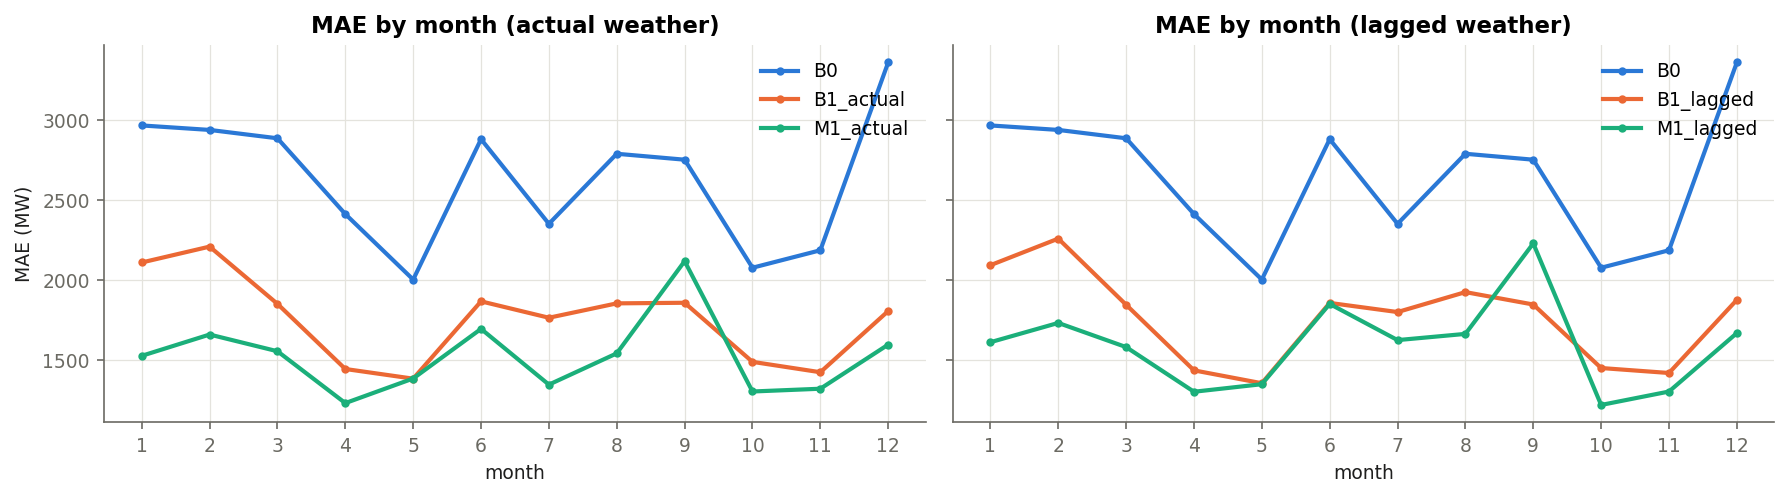
\includegraphics[width=\linewidth]{04_test_mae_by_month.png}
  \caption{Test MAE by month in both weather settings.}
  \label{fig:test-month}
\end{figure}

\paragraph{September 2018.} It is the only month in which LightGBM is clearly worse than Ridge
(\cref{fig:test-month}). The recorded load in early September does not follow the weekday pattern:
Saturday 1 and Sunday 2 September reach 34{,}064 and 34{,}646\,MW (higher than an ordinary
workday), while Thursday 6 and Wednesday 12 September are as low as a Sunday. The TSO forecast column
shows the same pattern within about 1\%, so these values are either real unusual events or a date
misalignment in the source; we cannot tell which. We did not change the test data. In a post-hoc
check (decided after seeing the results, so only supporting evidence), removing September keeps
all verdicts unchanged and widens the LightGBM gain to 275\,MW (actual) and 218\,MW (lagged).

\subsection{Separating Fitting, Features and Structure}
\label{sec:eval-ablation}

\paragraph{Protocol and disclosure.} The variants of \cref{tab:variants} were added \emph{after} the
test results above were known. Their configuration was chosen on validation only, frozen with
SHA-256 hashes and committed, and only then was 2018 loaded a second time, in one run, for these
models only. B0, B1 and M1 were not refitted, so all numbers above are unchanged. A first attempt of
this run stopped at its precondition check before reading any data. On validation the verdicts are
the same as in \cref{tab:ablation}, except that feature engineering for the global Ridge was
undecided in the lagged setting. These results are therefore supporting evidence, weaker than the
pre-registered comparison above.

\begin{table}[H]
  \centering
  \small
  \caption{Paired comparisons on the test year for the added variants ($\Delta=\MAE_A-\MAE_B$ in MW,
           95\% block-bootstrap interval). All verdicts are ``A clearly better'' unless noted.}
  \label{tab:ablation}
  \begin{tabular}{@{}l l r c r c@{}}
    \toprule
    & & \multicolumn{2}{c}{Actual} & \multicolumn{2}{c}{Lagged} \\
    \cmidrule(lr){3-4}\cmidrule(l){5-6}
    A & B & $\Delta$ & 95\% interval & $\Delta$ & 95\% interval \\
    \midrule
    \multicolumn{6}{@{}l}{\emph{Q1: fitting versus features}} \\
    Ridge F0, 24 models & B0 & $-665$ & $[-916,\,-421]$ & $-668$ & $[-917,\,-422]$ \\
    Ridge F1, 24 models (B1) & Ridge F0, 24 models & $-215$ & $[-298,\,-133]$ & $-204$ & $[-283,\,-130]$ \\
    Ridge F1, global & Ridge F0, global & $-135$ & $[-209,\,-63]$ & $-116$ & $[-189,\,-50]$ \\
    LightGBM F1, global (M1) & LightGBM F0, global & $-488$ & $[-617,\,-360]$ & $-430$ & $[-561,\,-302]$ \\
    \addlinespace
    \multicolumn{6}{@{}l}{\emph{Q2: LightGBM versus Ridge at matched features and structure}} \\
    LightGBM F1, global & Ridge F1, global & $-457$ & $[-576,\,-331]$ & $-401$ & $[-512,\,-288]$ \\
    LightGBM F1, 24 models & Ridge F1, 24 models & $-184$ & $[-284,\,-81]$ & $-167$ & $[-266,\,-64]$ \\
    LightGBM F0, global & Ridge F0, global & $-104$ & $[-161,\,-43]$ & $-87$ & $[-146,\,-26]$ \\
    \addlinespace
    \multicolumn{6}{@{}l}{\emph{Structure: 24 per-hour models versus one global model}} \\
    Ridge F1, 24 models & Ridge F1, global & $-226$ & $[-276,\,-177]$ & $-233$ & $[-284,\,-181]$ \\
    LightGBM F1, 24 models & LightGBM F1, global & $+48$ & $[1,\,93]$ & $+2$ & $[-54,\,58]$ \\
    \bottomrule
  \end{tabular}
  \par\smallskip\footnotesize Last row: B clearly better (actual), undecided (lagged).
\end{table}

\begin{itemize}
  \item \textbf{Q1: most of the B0$\to$B1 gain comes from fitting.} Ridge on B0's own information
        plus the calendar (F0) already removes 665--668\,MW. The engineered features remove a further
        204--215\,MW. Of the 880\,MW gap between B0 and B1, about three quarters is therefore due to
        fitting a model and one quarter to feature engineering. Both steps win in 12 of 12 months.
  \item \textbf{Features help LightGBM more than Ridge} (430--488\,MW versus 116--215\,MW). We did
        not test why. One plausible reason is that F1 adds information that is absent from F0
        (holidays, the most recent load), and that trees can combine it with hour and weekday,
        whereas Ridge can only add it linearly.
  \item \textbf{Q2: LightGBM beats Ridge in every matched pair}, by 401--457\,MW with one model each,
        167--184\,MW with 24 models each and 87--104\,MW on minimal features. The conclusion of
        \cref{tab:test-pairs} thus does not depend on the difference in structure, but the size of
        the gap does.
  \item \textbf{Each model is strongest in its own structure.} Splitting Ridge into 24 models
        removes about 230\,MW, because it is how a linear model gets hour-specific effects. Splitting
        LightGBM does not help (+48\,MW actual, clearly worse; +2\,MW lagged, undecided), consistent
        with each per-hour model seeing only 1/24 of the rows. The main comparison (B1 versus M1)
        therefore pits each model in the structure that suits it.
\end{itemize}

\subsection{Why Models Win or Lose}
\label{sec:eval-why}

\begin{table}[H]
  \centering
  \small
  \caption{Test MAE (MW) by day type and by temperature band (actual weather unless noted).}
  \label{tab:test-groups}
  \begin{tabular}{@{}l r r r r r@{}}
    \toprule
    Group & Hours & B0 & B1 & M1 & M1 $-$ B1 \\
    \midrule
    Workday & 5{,}926 & 2{,}494 & 1{,}662 & 1{,}416 & $-246$ \\
    Saturday & 1{,}200 & 2{,}469 & 1{,}680 & 1{,}617 & $-63$ \\
    Sunday & 1{,}246 & 3{,}020 & 2{,}102 & 1{,}723 & $-379$ \\
    Holiday & 264 & 4{,}777 & 2{,}567 & 2{,}272 & $-295$ \\
    Bridge day & 120 & 2{,}324 & 1{,}495 & 1{,}965 & $+469$ \\
    \midrule
    $T<5\,^\circ$C & 375 & 2{,}942 & 2{,}045 & 1{,}612 & $-432$ \\
    5--10\,$^\circ$C & 1{,}663 & 2{,}672 & 1{,}855 & 1{,}387 & $-468$ \\
    10--15\,$^\circ$C & 2{,}187 & 2{,}623 & 1{,}644 & 1{,}436 & $-208$ \\
    15--20\,$^\circ$C & 1{,}734 & 2{,}550 & 1{,}622 & 1{,}551 & $-70$ \\
    20--25\,$^\circ$C & 1{,}577 & 2{,}388 & 1{,}579 & 1{,}477 & $-102$ \\
    $T>25\,^\circ$C & 1{,}220 & 2{,}930 & 2{,}123 & 1{,}838 & $-285$ \\
    \bottomrule
  \end{tabular}
\end{table}

\begin{itemize}
  \item \textbf{Where LightGBM gains: cold and hot hours.} The gain over Ridge is largest below
        10\,$^\circ$C (430--470\,MW) and above 25\,$^\circ$C (285\,MW), and small in the mild range
        15--25\,$^\circ$C (70--100\,MW). The same holds in the lagged setting. This points to the
        temperature response: Ridge has one fixed V-shape per hour with a kink at 18\,$^\circ$C, while
        the trees can bend the response and combine it with month, weekday and the current load level.
        By month, the largest gains are in January--February (550--580\,MW).
  \item \textbf{Where LightGBM loses: bridge days.} On the 5 bridge days of 2018 (120 hours) the
        error of LightGBM is 469\,MW larger than that of Ridge. It forecasts too high, treating these
        days almost like normal workdays. On validation it also
        lost on holidays; on the test year it wins on holidays ($-295$\,MW). With only 10--11
        holiday days a year this difference is not stable; the bridge-day result appeared in both years.
  \item \textbf{Weather setting.} Knowing the actual weather helps LightGBM (71\,MW) but not Ridge
        ($-8$\,MW, undecided). Given the cold/hot pattern above, the trees seem to use same-day
        temperature in the extremes, which the degree-day form with fixed bases cannot.
\end{itemize}
These are associations found in the error breakdown, not proven causes.

\subsection{Model Explanation Results}
\label{sec:eval-shap}

Both LightGBM models chose the level target, so SHAP values explain the predicted load itself.

\begin{figure}[H]
  \centering
  \begin{subfigure}[b]{0.42\linewidth}
    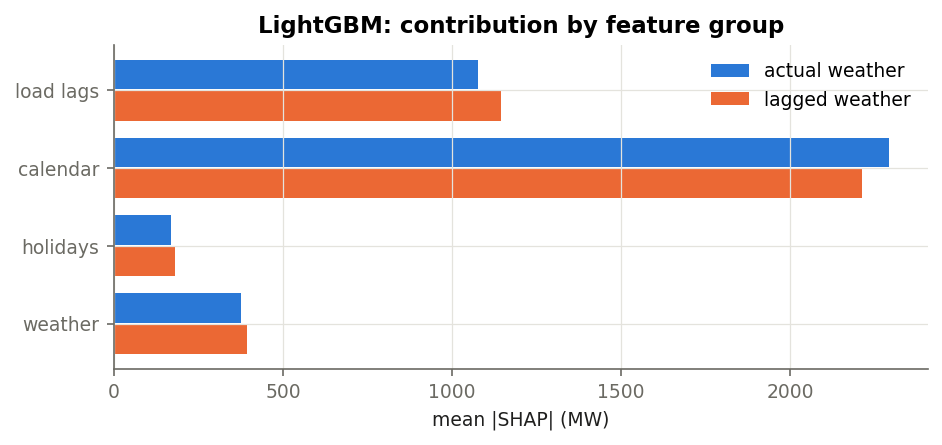
\includegraphics[width=\linewidth]{04_test_shap_groups.png}
    \caption{Mean $|\text{SHAP}|$ per feature group.}
  \end{subfigure}\hfill
  \begin{subfigure}[b]{0.56\linewidth}
    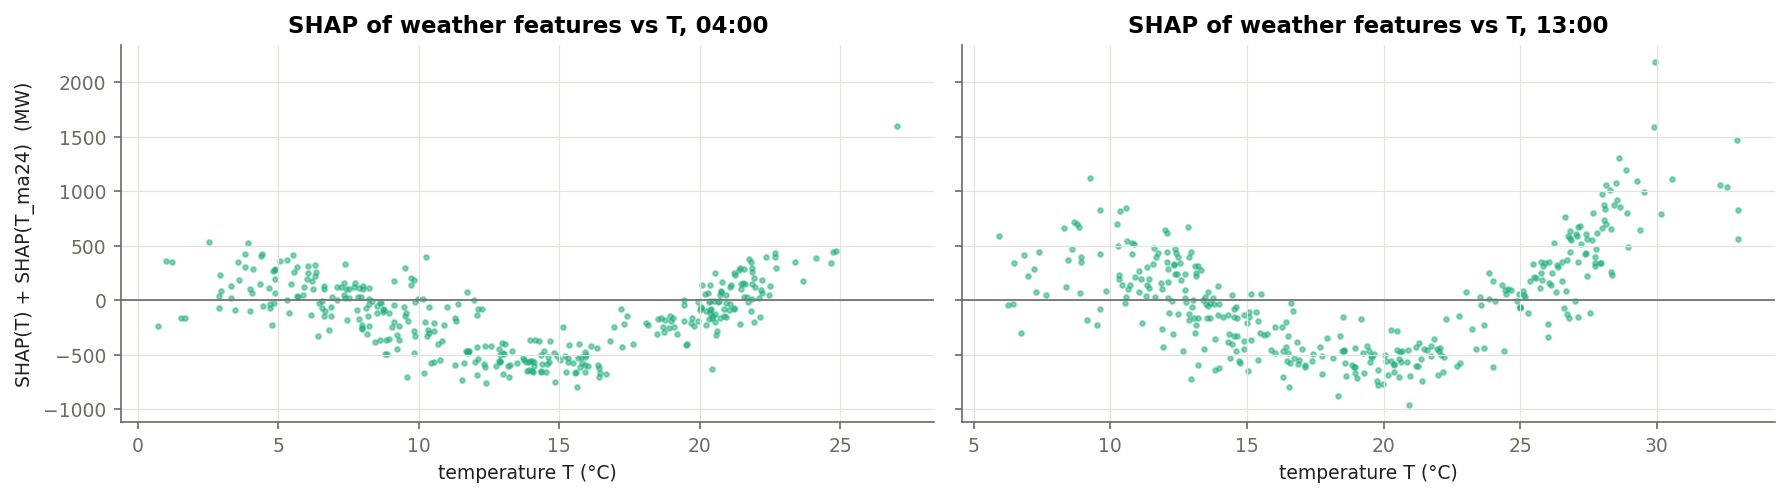
\includegraphics[width=\linewidth]{04_test_shap_temperature.png}
    \caption{Weather SHAP against temperature (actual).}
  \end{subfigure}
  \caption{SHAP explanation of LightGBM on the test year.}
  \label{fig:shap}
\end{figure}

\begin{itemize}
  \item \textbf{Calendar dominates} (mean $|$SHAP$|$ 2{,}292\,MW in the actual setting), mostly the
        hour of day (2{,}114\,MW) and weekday (698\,MW): the model first reproduces the daily and weekly
        shape. \textbf{Load lags} come second (1{,}077\,MW), then \textbf{weather} (375\,MW) and
        \textbf{holidays} (169\,MW). The lagged setting gives almost the same ranking, with more weight
        on $y_{D-7,h}$.
  \item \textbf{Weather} matters most in spring and late summer (482--554\,MW in April--May,
        512\,MW in August) and least in September and December (about 230--250\,MW).
  \item \textbf{Learned temperature response.} The weather SHAP has a clear U/V shape at both 04:00
        and 13:00, with its minimum around 15--20\,$^\circ$C and a steeper hot branch at midday
        (\cref{fig:shap}). This matches the V-shape with its kink at 18\,$^\circ$C that validation chose
        for Ridge, so the two models agree on the form of the response. Because temperature is
        correlated with season (\cref{tab:s2}), this shape describes what the model uses, not a causal
        effect of temperature.
\end{itemize}

\subsection{Comparison with the TSO Forecast}
\label{sec:eval-tso}

The TSO column has a test MAE of 268\,MW, about one sixth of our best model. It even follows the
unusual September days. This is consistent with the TSO using information we do not have (weather
forecasts, internal data, possibly updates after 10:00 on $D-1$). We report it only as context and
make no claim of beating or losing to it.

% =====================================================================
%  5. Discussion and future work
% =====================================================================
\section{Discussion and Future Work}
\label{sec:discussion}

\subsection{Discussion}
\label{sec:disc}

All answers below come from the single test run on 2018 and agree with validation 2017.

\paragraph{Q1: feature engineering with a linear model.} Ridge with lags, calendar, holiday and
degree-day features removes about a third of the seasonal-naive error (880\,MW, 3.0\% of mean load) in
every month of the test year. This is by far the largest single gain in the study.

\paragraph{Q2: a non-linear model.} LightGBM removes a further 13\% of the Ridge error with actual
weather (231\,MW) and 10\% with lagged weather (168\,MW), winning in 10--11 of 12 months. The gain is
concentrated in cold and hot hours and in winter months, i.e.\ where the response to temperature
and its interaction with calendar matter most. Ridge stays better on bridge days, and LightGBM lost
September 2018, a month with unusual recorded load.

\paragraph{Q3: knowing the actual weather.} With perfect knowledge of the day's temperature,
LightGBM improves by 71\,MW (0.25\% of load); Ridge does not improve measurably. This is an upper
bound for the value of weather forecasts in this set-up, and it is smaller than the gain from
changing the model. It agrees with the weak within-month temperature effect found on the training
years (\cref{tab:s2}): once lags and calendar are present, temperature adds little extra information.
This does not mean temperature is unimportant; much of its effect is already carried by the season
and by recent load.

\paragraph{What this means for a public-data analyst.} Spend effort first on features (lags at the
right information time, calendar, holidays), then on a flexible model; a weather-forecast feed comes
last for a national day-ahead forecast of this kind. Holidays and bridge days remain the weakest
point of every model and are the most promising place for further work. The TSO forecast is still
far more accurate (268\,MW), so a public-data model is useful for understanding and analysis, not as
a replacement.

\subsection{Limitations}
\label{sec:limitations}

\begin{itemize}
  \item \textbf{No weather forecasts.} Only an optimistic (actual) and a pessimistic (lagged) bound
        can be measured; operational performance lies in between.
  \item \textbf{Few seasons.} Training covers two summers when tuning and three when testing. The
        June 2017 heat wave shows that unseen extremes cause large bias, especially for trees, which
        cannot extrapolate.
  \item \textbf{Weather quality.} A simple five-city mean, no population weights; the origin of the
        weather data is not documented.
  \item \textbf{Holidays.} Regional holidays are only captured as an unweighted share of regions.
  \item \textbf{One test year,} one refit per year (the model may age during 2018), heuristic
        thresholds ($\delta$, spike rule, grids).
  \item \textbf{Actual load} may have been revised after publication; the TSO column's information
        time is unknown.
  \item \textbf{Tuning budgets differ:} 94 Ridge fits versus 30 LightGBM trials whose early stopping
        uses the same validation year. The resulting optimism of M1 on validation is estimated at
        10--30\,MW, small next to the 175--249\,MW gap. The chosen \code{min\_data\_in\_leaf} (11--13)
        lies near the lower edge (10) of the search space. The number of trees is kept fixed when
        refitting on three years, which, if anything, slightly disadvantages M1.
  \item \textbf{Design details:} the spike rule looks at the next hour, so in principle the
        cleaning of hour 08 on $D-1$ uses hour 09 (no spike fell on hour 08). In the actual setting,
        the 24-hour mean temperature at early hours of $D$ also uses the rest of $D-1$. The holiday
        table misses five national holidays that fell on a Sunday in 2015--2017 (none in 2018).
        The eight test comparisons are not corrected for multiple testing.
  \item All relations are statistical associations, not causal effects.
\end{itemize}

\subsection{Future Work}
\label{sec:future}

Items are ordered by expected value for the questions of this report. Status is updated as work
progresses.

\begin{table}[H]
  \centering
  \small
  \caption{Planned extensions (not done yet unless marked).}
  \label{tab:future}
  \begin{tabularx}{\linewidth}{@{}l Y l@{}}
    \toprule
    ID & Extension & Status \\
    \midrule
    F1 & Monthly refit on the test year (rolling origin) instead of one refit per year. & \todo{} \\
    F2 & Population-weighted temperature, or degree days per city before averaging. & \todo{} \\
    F3 & Diebold--Mariano test as a cross-check of the block bootstrap. & \todo{} \\
    F4 & Ridge without load lags (2$\times$2: with/without lags $\times$ with/without temperature) to
         see how much temperature information the lags absorb. & \todo{} \\
    F5 & Error breakdown with and without special days, to compare with studies that exclude
         them~\cite{incremona2021italian,dudek2021ensembles}. & \todo{} \\
    F6 & Cubic temperature terms and temperature $\times$ month for Ridge (is Ridge limited by its
         functional form?). & \todo{} \\
    F7 & Humidity as an extra weather variable (actual setting only). & \todo{} \\
    F8 & Similar-day (pattern-based) baseline~\cite{dudek2021ensembles}. & \todo{} \\
    F9 & Sensitivity to an earlier issue time ($D-2$) for both load and weather. & \todo{} \\
    F10 & A deep model (MLP or LSTM) under the same protocol, if the scope allows. & \todo{} \\
    F11 & Probabilistic forecasts (quantile LightGBM) for operational use. & \todo{} \\
    F12 & Better bridge-day handling (e.g.\ a bridge $\times$ hour interaction, or using the previous
          year's bridge days), the weakest point of LightGBM in both years. & \todo{} \\
    F13 & Check the unusual load of September 2018 against the original ENTSO-E data (real events
          or date misalignment?). & \todo{} \\
    \bottomrule
  \end{tabularx}
\end{table}


% =====================================================================
%  Required declarations and links  (placeholders - filled in by the group)
% =====================================================================
\section*{AI Usage Disclosure}
\addcontentsline{toc}{section}{AI Usage Disclosure}
\label{sec:ai-disclosure}

% TODO (group): tool(s) and version, member who used each tool, purpose, representative
% prompts or prompt-log link, affected sections/files, how outputs were edited and verified,
% member responsible for final verification, verification sources.
% Known so far: Claude Code (Anthropic) was used for the design debate (debate/), code in src/ and
% scripts/, and a first draft of this report.
We used Claude Opus 5.5 (Anthropic), through Claude Code, for the following tasks.
\begin{itemize}
  \item \textbf{Literature review.} The AI surveyed prior work on electricity load forecasting,
        from statistical methods to machine learning and deep learning, and suggested references.
        We verified every suggested reference against its original source before citing it.
  \item \textbf{Report structure and drafting.} We gave the AI the required outline
        (1~Problem Definition, 2~Literature Review, 3~Algorithm Implementation, 4~Evaluation,
        5~Discussion and Future Work, AI Usage Disclosure, Required Links) and asked it to set up
        the structure and write the main \LaTeX{} files.
  \item \textbf{Language editing.} Each member wrote one section, and the AI then edited its
        language for clarity and consistency.
  \item \textbf{Code, figures and slides.} The AI also helped write the analysis code in
        \code{src/} and \code{scripts/}, the figures, and the presentation slides. We ran the
        code and checked its outputs ourselves.
\end{itemize}
The group reviewed all AI output and takes full responsibility for the content of this report.


\section*{Required Links}
\addcontentsline{toc}{section}{Required Links}
\label{sec:links}

\begin{itemize}
  \item Source code repository: \url{https://github.com/pbt245/CO3135-Assignment}
  \item Kaggle notebooks / outputs: \url{https://www.kaggle.com/code/bathanhphan/p4aids-04-test}
\end{itemize}


\bibliographystyle{plainnat}
\bibliography{references}

\end{document}
